En la siguiente figura se indican las cuatro restricciones de un problema de programación lineal entera:

\begin{figure}[h!]
    \centering
    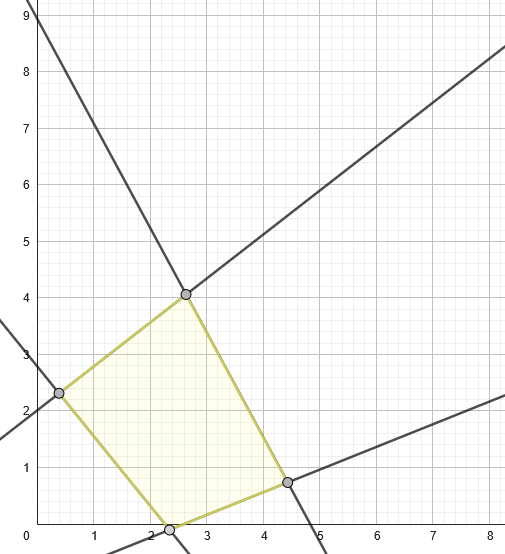
\includegraphics[width=10cm]{ejercicios/convex_hull_enunciado.png} 
\end{figure}

Formula las restricciones que generan el \textit{convex hull} (o envolvente convexa) de este problema.
